\documentclass[11pt,a4paper]{article}

% --- Packages ---
\usepackage[utf8]{inputenc}
\usepackage[T1]{fontenc}
\usepackage{lmodern}
\usepackage[margin=2.5cm]{geometry}
\usepackage{amsmath,amssymb}
\usepackage{graphicx}
\usepackage{booktabs}
\usepackage{array}
\usepackage{tikz}
\usetikzlibrary{arrows.meta,positioning,calc,fit,shapes.geometric,decorations.pathreplacing}
\usepackage[ruled,vlined,linesnumbered]{algorithm2e}
\usepackage{listings}
\usepackage{hyperref}
\usepackage{cleveref}
\usepackage{xcolor}
\usepackage{enumitem}
\usepackage{url}
\usepackage{bytefield}
\usepackage{multirow}

% --- Hyperref setup (PDF metadata) ---
\hypersetup{
  colorlinks=true,
  linkcolor=blue!70!black,
  citecolor=green!50!black,
  urlcolor=blue!70!black,
  pdftitle={Chameleon: A Polymorphic UDP Tunneling Protocol with Session-Unique Wire Formats},
  pdfauthor={william-aqn},
  pdfsubject={Polymorphic UDP tunneling protocol with per-session wire format derivation from PSK via HKDF-SHA256},
  pdfkeywords={UDP tunneling, protocol polymorphism, traffic obfuscation, deep packet inspection, AEAD encryption, network security},
  pdfcreator={LaTeX with hyperref},
}

% --- Listings setup ---
\lstset{
  basicstyle=\ttfamily\small,
  breaklines=true,
  frame=single,
  numbers=left,
  numberstyle=\tiny\color{gray},
  keywordstyle=\color{blue!70!black}\bfseries,
  commentstyle=\color{green!50!black}\itshape,
  stringstyle=\color{red!60!black},
  showstringspaces=false,
  tabsize=2,
}

% --- Custom commands ---
\newcommand{\chameleon}{\textsc{Chameleon}}
\newcommand{\genome}{\emph{genome}}
\newcommand{\psk}{\textsf{PSK}}
\newcommand{\field}[1]{\texttt{#1}}

\title{\textbf{Chameleon: A Polymorphic UDP Tunneling Protocol\\with Session-Unique Wire Formats}}
\author{william-aqn\\
  \small ORCID: \href{https://orcid.org/0009-0005-4749-1606}{0009-0005-4749-1606}\\
  \small \url{https://github.com/william-aqn/genome}
}
\date{April 2026}

\begin{document}
\maketitle

\vspace{-1em}
\noindent\rule{\textwidth}{0.4pt}
\smallskip
\noindent
\textbf{DOI:} \href{https://doi.org/10.5281/zenodo.19493212}{10.5281/zenodo.19493212} \hfill
\textbf{License:} \href{https://creativecommons.org/licenses/by/4.0/}{CC BY 4.0}\\
\noindent
\textbf{Source code:} \url{https://github.com/william-aqn/genome} \hfill
\textbf{Software license:} \href{https://www.gnu.org/licenses/gpl-3.0.html}{GPL-3.0}
\smallskip
\noindent\rule{\textwidth}{0.4pt}
\medskip

% ============================================================
\begin{abstract}
Deep packet inspection (DPI) systems identify tunneling protocols by matching fixed byte patterns, header structures, and handshake sequences. We present \chameleon{}, a polymorphic UDP tunneling protocol where each session deterministically derives a unique wire format---called a \genome{}---from a pre-shared key (PSK) via HKDF-SHA256. The derived genome controls the packet magic byte, header field ordering, number and size of decoy fields, nonce length, payload length encoding scheme, padding range, and (when stream mode is enabled) per-packet \emph{wagon} size range. A deterministic PRNG based on SHA-256 in counter mode ensures that both endpoints independently derive an identical genome without any handshake.

Wire output achieves approximately 7.9 bits per byte of Shannon entropy, making individual packets statistically indistinguishable from uniform random data. The protocol provides authenticated encryption via ChaCha20-Poly1305, XChaCha20-Poly1305, or AES-256-GCM, with epoch-based nonce construction and a 256-epoch anti-replay sliding window.

On top of the encrypted polymorphic transport, a stream multiplexer provides reliable, ordered delivery with selective acknowledgment (SACK), Jacobson/Karels RTT estimation, NewReno congestion control, and per-stream flow control. An optional \emph{stream mode} emits a constant flow of genome-shaped wagons at a configurable rate envelope, carrying real data when available and random chaff otherwise, defending against passive timing and activity inference on top of structural polymorphism. Empirical evaluation over a transatlantic link shows sustained throughput of 30~Mbit/s with 67 concurrent streams; stream mode preserves 86--97\% of direct throughput at its default 500~KB/s--3~MB/s envelope.

\chameleon{} is implemented in Go with a single external dependency (\texttt{golang.org/x/crypto}) and is available as open-source software under the GPL-3.0 license.
\end{abstract}

\paragraph{Keywords:} protocol polymorphism, traffic obfuscation, UDP tunneling, deep packet inspection evasion, AEAD encryption, stream multiplexing, cover traffic, traffic analysis resistance, censorship circumvention

% ============================================================
\section{Introduction}\label{sec:intro}

Network censorship increasingly relies on deep packet inspection (DPI) to identify and block circumvention tools. Modern DPI systems operate at line rate, matching protocol fingerprints against databases of known signatures. When a tunneling protocol uses fixed magic bytes, predictable header structures, or recognizable handshake patterns, these become reliable signatures for blocking.

Existing circumvention tools adopt two broad strategies. \emph{Protocol mimicry} disguises tunnel traffic as a permitted protocol (e.g., TLS, HTTP). While effective against simple blacklists, mimicry is fragile: even subtle deviations from the legitimate protocol's state machine, timing, or statistical properties can be detected by sophisticated DPI \cite{wang2012censorspoofer}. \emph{Randomization} approaches, such as obfs4 \cite{obfs4spec} and ScrambleSuit \cite{winter2013scramblesuit}, aim to produce uniformly random output. However, these tools still have fixed elements in their handshake or session establishment phase that can serve as fingerprints.

\chameleon{} takes a different approach: \emph{per-session polymorphism} of the entire wire format. Rather than randomizing payload bytes while keeping frame structure fixed, \chameleon{} derives a unique packet format for each session from a pre-shared key. The format itself---field order, field count, encoding schemes, and padding parameters---changes with every session. An observer who does not possess the PSK cannot predict the structure of any given packet, eliminating structural fingerprints entirely.

\paragraph{Contributions.} This paper makes the following contributions:
\begin{enumerate}[nosep]
  \item A \emph{genome derivation} mechanism that deterministically generates a complete wire format specification from a PSK using HKDF and a platform-stable PRNG (\cref{sec:genome}).
  \item A \emph{layered architecture} that cleanly separates polymorphic framing, authenticated encryption, reliable delivery, and stream multiplexing (\cref{sec:arch}).
  \item An \emph{epoch-based nonce} construction with anti-replay protection that eliminates nonce-reuse risks without per-packet random nonce generation (\cref{sec:crypto}).
  \item A reliable stream multiplexer over UDP with SACK, NewReno congestion control, and per-stream flow control (\cref{sec:mux}).
  \item A \emph{stream mode} (\cref{sec:stream}) that emits a constant, genome-shaped flow of ``wagons'' carrying real data or chaff. Per-packet wagon sizes are drawn from a genome-derived range $[W_{\min}, W_{\max}]$; the flow rate drifts inside an operator-configured envelope; burst mode drains the queue ``as is'' when real data exceeds the envelope.
  \item An \emph{empirical evaluation} demonstrating 30~Mbit/s throughput, 67 concurrent streams, wire entropy of 7.9 bits/byte, and 86--97\% goodput retention under stream mode (\cref{sec:eval}).
\end{enumerate}

The rest of this paper is organized as follows. \cref{sec:related} surveys related work. \cref{sec:arch} describes the system architecture. \cref{sec:genome} details the genome derivation mechanism. \cref{sec:crypto} covers the cryptographic layer. \cref{sec:mux} describes the stream multiplexer. \cref{sec:stream} introduces the stream (cover-traffic) mode. \cref{sec:security} presents the security analysis. \cref{sec:eval} reports performance results. \cref{sec:future} outlines future work, and \cref{sec:conclusion} concludes.

% ============================================================
\section{Related Work}\label{sec:related}

\paragraph{Tor pluggable transports.} The Tor Project introduced the pluggable transport framework to decouple transport obfuscation from the Tor protocol itself \cite{dingledine2004tor}. Notable transports include:
\begin{itemize}[nosep]
  \item \textbf{obfs4} \cite{obfs4spec}: Uses a Curve25519 handshake with Elligator~2 encoding \cite{bernstein2012elligator} to make the initial key exchange indistinguishable from random. Post-handshake, obfs4 applies NaCl secret-box encryption. However, the handshake phase has a fixed two-message structure that sophisticated DPI can detect through timing and length analysis.
  \item \textbf{ScrambleSuit} \cite{winter2013scramblesuit}: A predecessor to obfs4 that introduced polymorphic padding and session ticket authentication. ScrambleSuit's wire format is fixed once the session is established.
  \item \textbf{meek and Snowflake}: Domain-fronting and WebRTC-based transports that piggyback on legitimate cloud infrastructure. These are orthogonal to wire-format polymorphism and face distinct challenges (cost, latency, provider cooperation).
\end{itemize}

\paragraph{Shadowsocks and derivatives.} Shadowsocks \cite{shadowsocks} encrypts SOCKS5 traffic with stream ciphers (later AEAD). VMess \cite{vmess} adds a request/response structure and per-session key negotiation. While these tools encrypt payload, they retain fixed structural elements: Shadowsocks uses a deterministic IV-address prefix, and VMess has a recognizable command structure. Recent DPI systems have exploited these regularities.

\paragraph{Protocol mimicry.} Tools like FTE, Stegotorus, and CensorSpoofer \cite{wang2012censorspoofer} disguise traffic as HTTP, DNS, or other protocols. Mimicry is fundamentally limited by the difficulty of perfectly reproducing a complex protocol's state machine, timing characteristics, and semantic behavior.

\paragraph{Distinction of \chameleon{}.} Unlike obfs4 and ScrambleSuit, which have a fixed post-handshake wire format, \chameleon{} varies the \emph{entire} packet structure per session---including field order, field count, and encoding schemes. Unlike Shadowsocks/VMess, there is no fixed initial structure. Unlike protocol mimicry, \chameleon{} does not attempt to impersonate any specific protocol, instead producing uniformly random output. The zero-handshake design (both sides derive the genome independently from the PSK) eliminates the handshake-phase fingerprint that affects obfs4.

% ============================================================
\section{System Architecture}\label{sec:arch}

\chameleon{} is structured as a layered protocol stack. Each layer has a single responsibility and communicates with adjacent layers through well-defined interfaces.

\begin{figure}[htbp]
\centering
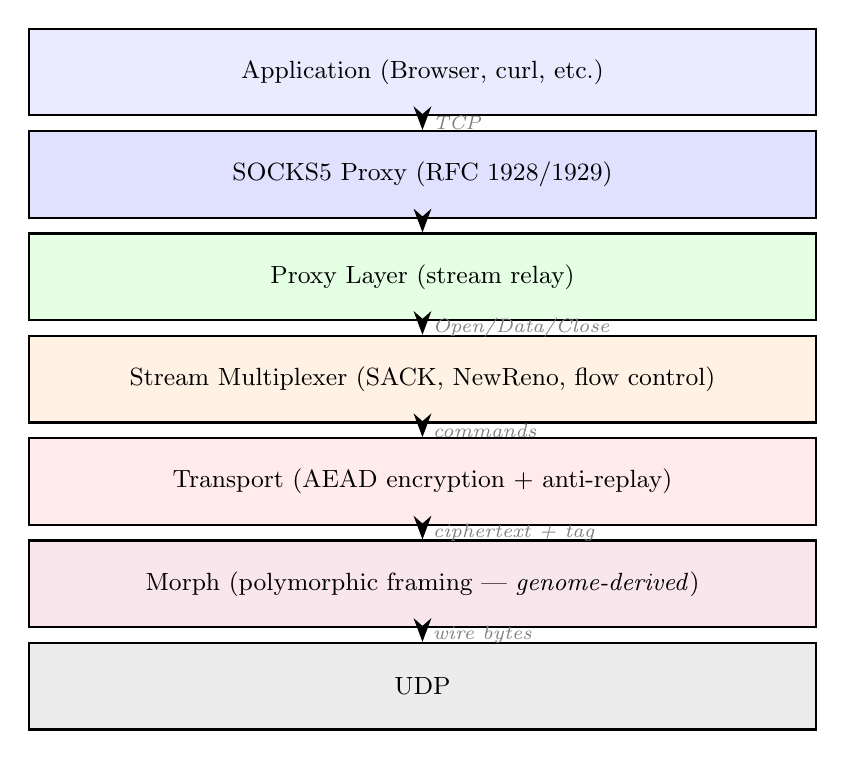
\begin{tikzpicture}[
  layer/.style={draw, thick, minimum width=10cm, minimum height=1.1cm, align=center, font=\small},
  arrow/.style={-{Stealth[length=3mm]}, thick},
  label/.style={font=\scriptsize\itshape, text=gray},
]
  % Layers
  \node[layer, fill=blue!8] (app) at (0,7) {Application (Browser, curl, etc.)};
  \node[layer, fill=blue!12] (socks) at (0,5.7) {SOCKS5 Proxy (RFC 1928/1929)};
  \node[layer, fill=green!10] (proxy) at (0,4.4) {Proxy Layer (stream relay)};
  \node[layer, fill=orange!10] (mux) at (0,3.1) {Stream Multiplexer (SACK, NewReno, flow control)};
  \node[layer, fill=red!8] (transport) at (0,1.8) {Transport (AEAD encryption + anti-replay)};
  \node[layer, fill=purple!10] (morph) at (0,0.5) {Morph (polymorphic framing --- \emph{genome-derived})};
  \node[layer, fill=gray!15] (udp) at (0,-0.8) {UDP};

  % Arrows
  \draw[arrow] (app) -- (socks) node[midway, right, label] {TCP};
  \draw[arrow] (socks) -- (proxy);
  \draw[arrow] (proxy) -- (mux) node[midway, right, label] {Open/Data/Close};
  \draw[arrow] (mux) -- (transport) node[midway, right, label] {commands};
  \draw[arrow] (transport) -- (morph) node[midway, right, label] {ciphertext + tag};
  \draw[arrow] (morph) -- (udp) node[midway, right, label] {wire bytes};
\end{tikzpicture}
\caption{Layered architecture of \chameleon{}. The morph layer derives its framing rules from the session genome, making the wire format unique per session.}
\label{fig:arch}
\end{figure}

\paragraph{Design principles.}
\begin{enumerate}[nosep]
  \item \textbf{Crypto-agnostic morph layer.} The morph layer handles frame serialization and deserialization but never invokes AEAD operations directly. The transport layer orchestrates both encryption and framing. This separation allows each layer to be tested independently.
  \item \textbf{Zero-handshake session establishment.} Both endpoints derive identical session keys and genome from the shared PSK without any key-exchange messages. This eliminates handshake-phase fingerprints and reduces latency.
  \item \textbf{Minimal dependencies.} The entire implementation depends only on \texttt{golang.org/x/crypto} for ChaCha20-Poly1305 and HKDF. All other functionality uses Go's standard library.
\end{enumerate}

% ============================================================
\section{Genome Derivation}\label{sec:genome}

The core novelty of \chameleon{} is the \emph{genome}---a complete specification of the wire format that is deterministically derived from the PSK. Two endpoints sharing the same PSK independently compute identical genomes, enabling communication without any negotiation.

\subsection{Key Hierarchy}\label{sec:keys}

Session keys are derived from the PSK using HKDF-SHA256 \cite{rfc5869}:

\begin{equation}\label{eq:hkdf}
  \text{PRK} = \text{HKDF-Extract}(\text{salt}, \text{PSK})
\end{equation}

Three values are expanded from the PRK using distinct info strings:

\begin{align}
  K_{\text{AEAD}} &= \text{HKDF-Expand}(\text{PRK},\; \texttt{"chameleon-aead-key"},\; 32) \label{eq:aead_key}\\
  S_{\text{genome}} &= \text{HKDF-Expand}(\text{PRK},\; \texttt{"chameleon-genome-seed"},\; 32) \label{eq:genome_seed}\\
  B_{\text{nonce}} &= \text{HKDF-Expand}(\text{PRK},\; \texttt{"chameleon-nonce-base"},\; 24) \label{eq:nonce_base}
\end{align}

where $K_{\text{AEAD}}$ is the 256-bit encryption key, $S_{\text{genome}}$ seeds the genome derivation, and $B_{\text{nonce}}$ provides the fixed prefix for nonce construction. The PSK must be at least 128 bits (16 bytes).

\subsection{Deterministic PRNG}\label{sec:prng}

Genome derivation requires a PRNG that is deterministic and platform-stable: the same seed must produce identical output regardless of Go version, operating system, or CPU architecture. The standard library's \texttt{math/rand} does not guarantee algorithm stability across versions.

\chameleon{} uses SHA-256 in counter mode:

\begin{equation}
  \text{block}_i = \text{SHA-256}(\text{seed} \;\|\; \text{counter}_i)
\end{equation}

where $\text{seed} = \text{SHA-256}(S_{\text{genome}})$ is the normalized 256-bit seed and $\text{counter}_i$ is a 64-bit little-endian counter starting at zero. Each invocation produces 32 bytes of pseudorandom output. The PRNG exposes the following operations used during derivation:

\begin{itemize}[nosep]
  \item $\texttt{Bytes}(n)$: returns $n$ pseudorandom bytes.
  \item $\texttt{Intn}(n)$: returns a uniform integer in $[0, n)$ using rejection sampling to eliminate modulo bias.
  \item $\texttt{Shuffle}(n, \text{swap})$: Fisher-Yates shuffle \cite{fisher1938statistical}.
\end{itemize}

\subsection{Genome Parameters}\label{sec:genome_params}

Given the PRNG seeded with $S_{\text{genome}}$, the genome $G$ is derived as follows:

\begin{enumerate}
  \item \textbf{Magic byte} ($m$): A single pseudorandom byte $m \in [0, 255]$ placed at position 0 of every packet. Acts as a fast-path filter: packets with a wrong magic byte are discarded without further processing.

  \item \textbf{Nonce size} ($n_s$): Either 12 or 24 bytes, selected uniformly. This determines the AEAD variant: 12-byte nonces use ChaCha20-Poly1305 or AES-256-GCM; 24-byte nonces use XChaCha20-Poly1305.

  \item \textbf{Length encoding} ($\ell$): One of four schemes, selected uniformly:
  \begin{itemize}[nosep]
    \item Big-endian \texttt{uint16} (2 bytes, fixed)
    \item Little-endian \texttt{uint16} (2 bytes, fixed)
    \item Unsigned varint (1--3 bytes, variable)
    \item XOR-masked big-endian \texttt{uint16} with a genome-derived 16-bit mask $\mu$ (2 bytes, fixed)
  \end{itemize}

  \item \textbf{Core fields}: Five mandatory fields are always present:
  \begin{itemize}[nosep]
    \item \field{Nonce}: $n_s$ bytes
    \item \field{Length}: encoded payload length (scheme-dependent)
    \item \field{PadLen}: 1 byte (padding length)
    \item \field{Tag}: 16 bytes (AEAD authentication tag)
    \item \field{Epoch}: 4 bytes (anti-replay counter, big-endian)
  \end{itemize}

  \item \textbf{Decoy fields} ($d$): Between 0 and 3 additional fields, each with a random size in $[1, 8]$ bytes. Each decoy has a genome-derived XOR mask; on the wire, decoy bytes are random data XORed with the mask. Decoys are indistinguishable from real fields without knowledge of the genome.

  \item \textbf{Field order}: All $5 + d$ fields are shuffled using Fisher-Yates with the genome PRNG, producing a permutation $\pi$.

  \item \textbf{Padding range} ($p_{\min}, p_{\max}$): $p_{\min} \in [0, 15]$, $p_{\max} \in [p_{\min}+1,\; p_{\min}+64]$. Each packet is padded with a random number of bytes drawn uniformly from $[p_{\min}, p_{\max}]$ using \texttt{crypto/rand}.

  \item \textbf{Wagon size range} ($W_{\min}, W_{\max}$): $W_{\min} = \text{MSS} + 16 + r_1$ with $r_1 \in [0, 15]$, and $W_{\max} = W_{\min} + 24 + r_2$ with $r_2 \in [0, 79]$. Used only when stream mode is enabled (\cref{sec:stream}); both endpoints derive the same range, so they agree on the envelope without negotiation. The constraint $W_{\min} \geq \text{MSS} + 2$ ensures that any mux-layer command fits in the shortest wagon with the 2-byte real-length prefix.
\end{enumerate}

\begin{table}[htbp]
\centering
\caption{Genome parameters and their derivation.}
\label{tab:genome}
\begin{tabular}{@{}llll@{}}
\toprule
\textbf{Parameter} & \textbf{Range} & \textbf{Derivation} & \textbf{Purpose} \\
\midrule
Magic byte $m$ & $[0, 255]$ & \texttt{Bytes(1)} & Packet identification \\
Nonce size $n_s$ & $\{12, 24\}$ & \texttt{Intn(2)} & AEAD variant selection \\
Length encoding $\ell$ & $\{0,1,2,3\}$ & \texttt{Intn(4)} & Header obfuscation \\
XOR mask $\mu$ & $[0, 65535]$ & \texttt{Uint32()} & Length field masking \\
Decoy count $d$ & $[0, 3]$ & \texttt{Intn(4)} & Field count variation \\
Decoy sizes & $[1, 8]$ each & \texttt{Intn(8)+1} & Field size variation \\
Field order $\pi$ & $(5+d)!$ perms & \texttt{Shuffle} & Structure randomization \\
Pad min $p_{\min}$ & $[0, 15]$ & \texttt{Intn(16)} & Minimum padding \\
Pad max $p_{\max}$ & $[p_{\min}+1, p_{\min}+64]$ & \texttt{Intn(64)+1} & Maximum padding \\
Wagon min $W_{\min}$ & $[\text{MSS}{+}16, \text{MSS}{+}31]$ & \texttt{MSS+16+Intn(16)} & Min wagon plaintext size \\
Wagon max $W_{\max}$ & $[W_{\min}{+}24, W_{\min}{+}103]$ & \texttt{Intn(80)+24} & Max wagon plaintext size \\
\bottomrule
\end{tabular}
\end{table}

\subsection{Combinatorial Diversity}\label{sec:diversity}

The total number of distinct genomes can be bounded as follows:

\begin{equation}\label{eq:diversity}
|G| = 256 \times 2 \times 4 \times \sum_{d=0}^{3} \left(\binom{4}{1}^{?} \cdot 8^d \cdot (5+d)! \cdot 16 \cdot 64\right)
\end{equation}

More precisely:
\begin{align}
|G| &= 256 \cdot 2 \cdot 4 \cdot 16 \cdot 64 \cdot \sum_{d=0}^{3} 8^d \cdot (5+d)! \nonumber \\
    &= 2{,}097{,}152 \cdot (120 + 8 \cdot 720 + 64 \cdot 5040 + 512 \cdot 40320) \nonumber \\
    &= 2{,}097{,}152 \cdot (120 + 5{,}760 + 322{,}560 + 20{,}643{,}840) \nonumber \\
    &= 2{,}097{,}152 \cdot 20{,}972{,}280 \nonumber \\
    &\approx 4.4 \times 10^{13} \label{eq:diversity_result}
\end{align}

This does not account for the XOR mask (an additional $2^{16}$ factor when XOR encoding is selected) or decoy XOR masks. The effective diversity exceeds $10^{13}$ distinct wire formats, making signature-based detection infeasible.

\subsection{Wire Format}\label{sec:wire}

Each packet on the wire has the following structure:

\begin{center}
\begin{bytefield}[bitwidth=1.2em]{32}
  \bitheader{0-31} \\
  \bitbox{8}{Magic} & \bitbox{24}{Header fields in permuted order $\pi$} \\
  \wordbox{1}{Header fields (continued, variable length)} \\
  \wordbox{1}{Ciphertext (variable length)} \\
  \wordbox{1}{Padding ($p_{\min}$ to $p_{\max}$ random bytes)}
\end{bytefield}
\end{center}

The header fields are serialized according to the permutation $\pi$ determined by the genome. An observer without the PSK cannot determine where one field ends and another begins, as field boundaries depend on the genome-derived order and sizes.

% ============================================================
\section{Cryptographic Layer}\label{sec:crypto}

\subsection{Authenticated Encryption}

\chameleon{} supports three AEAD constructions \cite{rfc5116}:
\begin{itemize}[nosep]
  \item \textbf{ChaCha20-Poly1305} \cite{rfc8439}: 256-bit key, 96-bit nonce (the default).
  \item \textbf{XChaCha20-Poly1305}: 256-bit key, 192-bit nonce. Selected when the genome specifies $n_s = 24$.
  \item \textbf{AES-256-GCM}: 256-bit key, 96-bit nonce. Available as a configuration option for hardware-accelerated environments.
\end{itemize}

All three produce a 128-bit (16-byte) authentication tag. The tag is placed as a separate field in the genome-defined header (not appended to ciphertext as in standard AEAD usage), further obscuring the packet structure.

\subsection{Epoch-Based Nonce Construction}\label{sec:nonce}

Traditional AEAD usage generates random nonces or uses sequential counters appended to ciphertext. \chameleon{} constructs nonces from a genome-derived base and a monotonic epoch counter:

\begin{equation}\label{eq:nonce}
  \text{Nonce}[0 \ldots n_s{-}5] = B_{\text{nonce}}[0 \ldots n_s{-}5], \quad
  \text{Nonce}[n_s{-}4 \ldots n_s{-}1] = \text{epoch}
\end{equation}

where $\text{epoch}$ is a 32-bit big-endian counter incremented with each packet. The epoch is also included in the AEAD associated data to bind the ciphertext to its position in the sequence.

This construction provides two guarantees:
\begin{enumerate}[nosep]
  \item \textbf{No nonce reuse}: The epoch is monotonically increasing. Combined with the genome-derived prefix, each nonce is unique within and across sessions (with overwhelming probability).
  \item \textbf{No random nonce transmission}: The nonce base is derived from the PSK; only the 4-byte epoch varies per packet, saving bandwidth compared to transmitting full random nonces.
\end{enumerate}

\subsection{Anti-Replay Protection}\label{sec:replay}

The receiver maintains a sliding window bitmap of size $W = 256$ epochs. The check proceeds as:

\begin{algorithm}[H]
\SetAlgoLined
\KwIn{Received epoch $e$, current maximum $e_{\max}$, bitmap $B[0\ldots W{-}1]$}
\KwOut{Accept or reject}
\If{$e = 0$}{
  \Return reject \tcp*{Epoch 0 is reserved}
}
\If{$e > e_{\max}$}{
  Shift window: clear bits for $[e_{\max}+1, e]$\;
  $e_{\max} \leftarrow e$\;
  Mark $B[e \bmod W]$\;
  \Return accept\;
}
\If{$e_{\max} - e \geq W$}{
  Reset window \tcp*{Client reconnected with new initial epoch}
  \Return accept\;
}
\If{$B[e \bmod W]$ is set}{
  \Return reject \tcp*{Duplicate packet}
}
Mark $B[e \bmod W]$\;
\Return accept\;
\caption{Anti-replay check with sliding window.}
\label{alg:replay}
\end{algorithm}

Each tunnel session begins with a random initial epoch (drawn from the upper half of the 32-bit range) to prevent replay window collisions when a client reconnects to a running server.

% ============================================================
\section{Reliable Stream Multiplexing}\label{sec:mux}

\chameleon{} multiplexes multiple bidirectional streams over a single UDP tunnel. The multiplexer provides reliable, ordered delivery on a per-stream basis, similar to TCP but over UDP.

\subsection{Commands}\label{sec:commands}

Four command types are defined:

\begin{table}[htbp]
\centering
\caption{Multiplexer command types.}
\label{tab:commands}
\begin{tabular}{@{}clp{7cm}@{}}
\toprule
\textbf{Code} & \textbf{Command} & \textbf{Fields} \\
\midrule
\texttt{0x01} & \textsc{Open} & StreamID (4B), Port (2B), AddrLen (2B), Addr (var) \\
\texttt{0x02} & \textsc{Data} & StreamID (4B), Seq (4B), Payload (var) \\
\texttt{0x03} & \textsc{Close} & StreamID (4B) \\
\texttt{0x04} & \textsc{Ack} & StreamID (4B), AckSeq (4B), Window (4B), NumSACK (2B), SACK blocks (8B each) \\
\bottomrule
\end{tabular}
\end{table}

Stream IDs use an odd/even allocation scheme: the client allocates odd IDs (1, 3, 5, \ldots) and the server allocates even IDs (2, 4, 6, \ldots). This eliminates the need for ID negotiation.

\subsection{Selective Acknowledgment}\label{sec:sack}

Each \textsc{Ack} command carries:
\begin{itemize}[nosep]
  \item A \emph{cumulative} acknowledgment number (all data up to this sequence number has been received).
  \item A \emph{receive window} advertisement (bytes the receiver is willing to accept).
  \item Zero or more \emph{SACK blocks}, each specifying a contiguous range $[\text{left}, \text{right})$ of received out-of-order data.
\end{itemize}

SACK blocks enable the sender to retransmit only the specific segments that were lost, rather than retransmitting everything from the cumulative ACK point forward.

\subsection{RTT Estimation}\label{sec:rtt}

Round-trip time is estimated using the Jacobson/Karels algorithm \cite{jacobson1988congestion}:

\begin{align}
  \text{RTTVAR} &\leftarrow \tfrac{3}{4}\,\text{RTTVAR} + \tfrac{1}{4}\,|\text{SRTT} - R| \\
  \text{SRTT} &\leftarrow \tfrac{7}{8}\,\text{SRTT} + \tfrac{1}{8}\,R \\
  \text{RTO} &= \text{SRTT} + 4 \cdot \text{RTTVAR}, \quad \text{clamped to } [200\text{ms}, 60\text{s}]
\end{align}

where $R$ is a new RTT sample. Karn's algorithm is applied: only segments that have not been retransmitted contribute to RTT samples, preventing ambiguous measurements from corrupting the estimator.

\subsection{Congestion Control}\label{sec:congestion}

The multiplexer implements NewReno congestion control \cite{rfc6582} with the following parameters:

\begin{table}[htbp]
\centering
\caption{Congestion control parameters.}
\label{tab:congestion}
\begin{tabular}{@{}lrl@{}}
\toprule
\textbf{Parameter} & \textbf{Value} & \textbf{Rationale} \\
\midrule
Initial CWND & 256 KB & Avoid starving parallel streams in slow start \\
Minimum CWND & 32 KB & Prevent collapse after loss \\
Maximum CWND & 16 MB & Full utilization on fast links \\
MSS & 1,200 B & Fits within typical UDP MTU budget \\
\bottomrule
\end{tabular}
\end{table}

\paragraph{Slow start.} CWND increases by the number of acknowledged bytes per ACK, approximately doubling per RTT.

\paragraph{Congestion avoidance.} CWND increases by $\text{MSS} \times \text{ackedBytes} / \text{CWND}$ per ACK, achieving approximately one MSS increase per RTT (additive increase).

\paragraph{Fast recovery.} Upon detecting three duplicate ACKs, the sender sets $\text{ssthresh} = \text{CWND}/2$, then $\text{CWND} = \text{ssthresh} + 3 \times \text{MSS}$. The sender retransmits the oldest unacknowledged segment and remains in recovery until an ACK advances the cumulative acknowledgment.

\paragraph{Timeout.} If the RTO expires before an ACK arrives, $\text{ssthresh} = \text{CWND}/2$ and $\text{CWND} = \text{minCWND}$. The RTO is doubled (exponential backoff).

\subsection{Per-Stream Flow Control}\label{sec:flow}

Each stream maintains an independent flow controller with a default receive window of 4~MB (maximum 64~MB). The receive window is advertised in every \textsc{Ack} command. Flow control is advisory: the receiver never drops data that exceeds the window, but the sender throttles its output when the advertised window is insufficient.

On the send side, each stream limits outstanding (unacknowledged) bytes to 256~KB. This serves as a send-side flow control that naturally paces UDP packets, preventing burst drops that occur when thousands of small packets are sent in rapid succession.

\subsection{Delayed Acknowledgment}\label{sec:delayed_ack}

To reduce ACK overhead, the multiplexer sends ACKs every 32 received data packets rather than per-packet. A 200~ms timer ensures that pending ACKs are flushed even during low-activity periods. ACKs are also triggered immediately when the receive window drops below 25\% of its default value.

% ============================================================
\section{Stream Mode: Constant-Rate Cover Traffic}\label{sec:stream}

\subsection{Motivation: Timing and Activity Inference}\label{sec:stream_motivation}

Structural polymorphism (\cref{sec:genome}) defeats signature-based DPI by making each packet statistically indistinguishable from random. However, a passive observer recording the \emph{flow-level} pattern---packet arrival times and counts---can still infer \emph{when} a user is active, even without decrypting a single byte. This ability enables website fingerprinting \cite{cai2012touching,panchenko2016website}, flow correlation across hops \cite{nasr2018deepcorr}, and statistical traffic analysis \cite{wright2009morphing}. Efficient countermeasures have historically been difficult to deploy without prohibitive cost \cite{dyer2012peekaboo}.

A natural defense is \emph{constant-rate cover traffic}: emit packets at a rate that is independent of application activity, so the observer sees no correlation between the encrypted flow and real events. \chameleon{}'s stream mode implements this defense while remaining consistent with the polymorphic-per-session design. Instead of a single fixed rate, \chameleon{} ties all observable cover parameters---packet size, flow rate envelope, burst thresholds---to the session genome, so that an observer without the PSK cannot even enumerate the envelope used by a particular session.

\subsection{Wagon Wire Format}\label{sec:wagon_format}

When stream mode is enabled, the plaintext carried inside the AEAD seal of every packet is a \emph{wagon}: a length-prefixed container of fixed size. The layout is:

\begin{center}
\begin{bytefield}[bitwidth=1.2em]{32}
  \bitheader{0-31} \\
  \bitbox{16}{\textsf{RealLen} (uint16 BE)} & \bitbox{16}{\textsf{Real bytes} (up to \textsf{RealLen})} \\
  \wordbox{1}{\textsf{Real bytes} (continued)} \\
  \wordbox{1}{Filler (zero bytes to total wagon size $W$)}
\end{bytefield}
\end{center}

\textsf{RealLen} is a 16-bit big-endian length. A value of zero marks a pure-chaff wagon; the receiver silently discards the entire plaintext. A nonzero value names the number of real mux-command bytes immediately following; the filler tail is left as zeros because AEAD output is already indistinguishable from random on the wire, and the receiver never inspects the filler (it reads only \textsf{RealLen} and the first \textsf{RealLen} bytes that follow). This saves a \texttt{crypto/rand} syscall on every packet.

Both endpoints use the wagon layout symmetrically; stream mode is an opt-in setting on each side, and peers must agree.

\subsection{Genome-Derived Wagon Sizes}\label{sec:wagon_sizes}

For each outgoing packet the sender draws a wagon size $W$ uniformly from $[W_{\min}, W_{\max}]$, where $W_{\min}$ and $W_{\max}$ are the genome-derived bounds introduced in \cref{sec:genome_params}. This gives three simultaneous properties:

\begin{enumerate}[nosep]
  \item \textbf{Per-packet variation.} Every wagon has a different plaintext size (up to ciphertext-length variation), so an observer cannot exploit a fixed-size signature or exact-size correlation across packets.
  \item \textbf{Genome-bound envelope.} Both $W_{\min}$ and $W_{\max}$ are HKDF-derived from the PSK. Only a peer who knows the PSK can predict the envelope. An observer sees random sizes but cannot determine the underlying range.
  \item \textbf{Asynchronous agreement.} The sender draws $W$ locally; the receiver does not need to predict it (the UDP datagram boundary carries the size). Packet loss or reordering does not desynchronize any shared PRNG state---there is none.
\end{enumerate}

The invariant $W_{\min} \geq \text{MSS} + 2$ guarantees that the largest mux command (a \textsc{Data} segment with a 1200-byte payload plus 9-byte header) fits inside the smallest possible wagon with its 2-byte prefix. No mux-layer fragmentation is required.

\subsection{Rate Envelope with Random Walk Drift}\label{sec:rate_envelope}

The emission rate is controlled by a single pump goroutine on each side, configured with operator-chosen bounds $R_{\min}$ and $R_{\max}$ in plaintext bytes per second. On a per-session basis the pump maintains a current target rate $R(t)$ that is nudged once per second by a reflected random walk:

\begin{equation}\label{eq:rate_drift}
  R(t+1) = \text{clamp}_{[R_{\min}, R_{\max}]}\!\left(R(t) + \Delta\right), \quad \Delta \sim \mathcal{U}\!\left(-\tfrac{R_{\max}-R_{\min}}{8},\; +\tfrac{R_{\max}-R_{\min}}{8}\right)
\end{equation}

Between drift updates the pump schedules its next emission at

\begin{equation}\label{eq:next_send}
  t_{\text{next}} = t_{\text{prev}} + \frac{W}{R(t)},
\end{equation}

where $W$ is the wagon size chosen for the packet. When the envelope is wider than typical real-traffic rates, the flow rate appears to drift irregularly inside the envelope even under a steady load---described informally as ``a river that is never at full flow''. This non-trivial rate variation, together with genome-varied wagon sizes, complicates simple volume-versus-time fingerprinting.

Wagon size $W$ is drawn at every tick, so the \emph{byte rate} follows $R(t)$ while the \emph{packet rate} is slightly modulated by the wagon-size distribution.

\subsection{Burst: Handling Real Data That Exceeds the Envelope}\label{sec:burst}

Constant-rate cover naturally conflicts with large downloads: if application bytes arrive faster than $R_{\max}$, something must give. The protocol's pump resolves this with a bounded \emph{burst mode}.

The mux layer pushes encoded commands into a queue of capacity $Q = 1024$ wagons. The pump tracks the queue depth $q$ with hysteresis:

\begin{align}
  q \geq Q_{\text{high}} \Rightarrow \text{enter burst}, \qquad & Q_{\text{high}} = 128 \\
  q \leq Q_{\text{low}}  \Rightarrow \text{exit burst},  \qquad & Q_{\text{low}}  = 32
\end{align}

In burst mode the effective rate used in \eqref{eq:next_send} is replaced by $R_{\text{burst}} = \beta \cdot R_{\max}$ with $\beta = 4$. This preserves a \emph{hard cap} on the wire rate---essential to avoid overrunning kernel UDP buffers, which would otherwise manifest as packet loss and trigger mux retransmissions that can collapse the stream---while allowing throughput to rise above the cover envelope when real data demands it. Both the hysteresis and $\beta$ are empirically tuned; see \cref{sec:eval_stream}.

The queue capacity is large enough that mux backpressure (through blocking \texttt{Enqueue}) engages only after burst has been active long enough to make meaningful headway, avoiding an oscillation in which mux-layer write throttling and pump drain rate alternately dominate.

\subsection{Pump Architecture and Single-Writer Model}\label{sec:pump_arch}

With no pump attached, many mux goroutines may call \texttt{Tunnel.Send} concurrently; \texttt{*net.UDPConn} serializes writes at the socket level but packet order is otherwise unspecified. With a pump attached, a single pump goroutine is the sole writer to the UDP socket. This gives three desirable properties at no cost:

\begin{enumerate}[nosep]
  \item Strictly ordered emissions (the ordering on the wire follows the pump's timing, not the mux's producer threads).
  \item No cross-goroutine interleaving of packets.
  \item Cadence that tracks $R(t)$ with no jitter introduced by producer scheduling.
\end{enumerate}

The pump holds a scratch buffer of $W_{\max}$ bytes that is reused across ticks; only the real-data \texttt{copy} is needed per packet, with zeroing of the filler tail via \texttt{clear}. A server pump also checks peer availability before emitting: until the server has discovered its first valid client packet (from which it learns the peer address) the pump preserves its cadence but emits no packets, avoiding log spam and wasted wire bytes.

\subsection{Cover Properties}\label{sec:cover_properties}

The combined effect of the above mechanisms is:

\begin{itemize}[nosep]
  \item In the \emph{idle regime}, packets flow at rate $R(t) \in [R_{\min}, R_{\max}]$ with genome-varying sizes; content is pure chaff but encrypted and indistinguishable from real traffic.
  \item In the \emph{partial-load regime} (aggregate real data below $R_{\max}$), real bytes replace filler within the same envelope; the wire rate is identical to the idle regime.
  \item In the \emph{full-load regime} (real data above $R_{\max}$), burst lifts the rate up to $\beta R_{\max}$, wagons are packed to the brim with real bytes, and filler shrinks toward zero. The rate increase reveals \emph{that} the user is pushing data but not what or where.
\end{itemize}

Narrowing the envelope (e.g., setting $R_{\min} = R_{\max} = 100$~KB/s) gives strict cover traffic at the cost of bounded throughput; widening it (e.g., $500$~KB/s--$3$~MB/s, the default) balances practical usability with continued indistinguishability of browsing versus idle activity. The operator chooses the tradeoff.

% ============================================================
\section{Security Analysis}\label{sec:security}

\subsection{Threat Model}\label{sec:threat}

We consider three adversary types:

\begin{enumerate}[nosep]
  \item \textbf{Passive observer with DPI}: Can observe all packets between client and server, perform statistical analysis, and match against known protocol signatures.
  \item \textbf{Active prober}: Can send crafted packets to the server to elicit recognizable responses.
  \item \textbf{Replay attacker}: Can record and retransmit previously observed packets.
\end{enumerate}

We assume the adversary does not possess the PSK.

\subsection{Resistance to Passive Analysis}

\paragraph{Structural fingerprinting.} Traditional DPI matches fixed byte patterns (e.g., TLS record type at byte 0, HTTP method at bytes 0--3). In \chameleon{}, the magic byte, field order, and field sizes change per session. The probability that two sessions share the same genome is at most $|G|^{-1} \approx 2.3 \times 10^{-14}$ (\cref{eq:diversity_result}), making it infeasible to build a structural signature.

\paragraph{Entropy analysis.} Each packet's output is designed to be indistinguishable from uniform random data. The encrypted payload (ChaCha20-Poly1305 or AES-GCM output) has near-maximal entropy by construction. Padding bytes are generated from \texttt{crypto/rand}. Decoy fields are random bytes XORed with genome-derived masks, producing uniformly distributed output.

We measure Shannon entropy $H$ over the byte distribution of wire output:
\begin{equation}
  H = -\sum_{i=0}^{255} p_i \log_2 p_i
\end{equation}

Empirical measurements on captured traffic yield $H \geq 7.9$ bits/byte (maximum is 8.0 for uniform distribution), confirmed by the entropy test in the test suite (\texttt{TestFrameEntropy}).

\paragraph{Length analysis.} Variable-length padding ($[p_{\min}, p_{\max}]$ bytes per packet) masks payload lengths. The four different length encoding schemes further complicate length-based correlation across sessions.

\subsection{Resistance to Active Probing}

The server processes a received packet through the following pipeline:
\begin{enumerate}[nosep]
  \item Magic byte check (immediate discard on mismatch).
  \item Morph decode (fails without correct genome).
  \item Anti-replay check (rejects duplicate/out-of-window epochs).
  \item AEAD decryption (fails without correct key).
\end{enumerate}

An active prober without the PSK fails at step~1 with probability $255/256 \approx 99.6\%$ and at step~4 with certainty (AEAD forgery is computationally infeasible). The server never sends a response to invalid packets, revealing no information to the prober.

\subsection{Replay Protection}

The 256-epoch sliding window (\cref{alg:replay}) rejects duplicate packets. The random initial epoch prevents an attacker from precomputing a valid epoch sequence. Even if an attacker replays a valid packet from a previous session, it will fail AEAD decryption because the session keys (derived from the same PSK but potentially different salt) differ.

\subsection{Resistance to Timing and Activity Inference}\label{sec:timing_analysis}

Without stream mode, \chameleon{} inherits the flow-level fingerprinting weakness common to all randomization-based tunnels: even with uniformly random packet content, \emph{when} a packet is sent is correlated with real application activity. Website fingerprinting attacks \cite{cai2012touching,panchenko2016website} and flow correlation attacks \cite{nasr2018deepcorr} exploit precisely this signal.

Stream mode (\cref{sec:stream}) attacks this signal directly:
\begin{enumerate}[nosep]
  \item In the idle and partial-load regimes, the wire rate is completely independent of application activity. An observer cannot distinguish a user browsing a news site from a user with no real traffic at all.
  \item In the full-load regime, the observer learns that the user is producing bytes at a rate above $R_{\max}$, but not the content, destination, or flow boundaries. This is analogous to observing a VPN user's aggregate bandwidth without learning what sites they visit.
  \item Per-packet sizes are drawn from the genome-derived envelope $[W_{\min}, W_{\max}]$; only a peer with the PSK can predict the range. Size-based attacks such as the ones in \cite{dyer2012peekaboo} require stable size distributions, which \chameleon{} denies by tying them to the session PSK.
\end{enumerate}

Operators seeking stricter cover can narrow the envelope, at the cost of throughput. The protocol does not attempt to hide that \emph{some} cover traffic is flowing---that would require a complete blending attack against a host protocol---but it hides \emph{when} the user is active.

\subsection{Known Limitations}\label{sec:limitations}

\begin{enumerate}[nosep]
  \item \textbf{High-entropy detection.} An adversary who blocks \emph{all} high-entropy traffic (the ``noise paradox'') would also block \chameleon{}. This is a fundamental limitation of any randomization-based approach.
  \item \textbf{No forward secrecy.} Without an ephemeral key exchange (e.g., ECDH), compromise of the PSK allows decryption of all past and future sessions.
  \item \textbf{Cover breach during burst.} When real traffic exceeds the envelope, the pump's burst mode lifts the wire rate above $R_{\max}$, visibly signaling heavy activity. Narrow envelopes trade throughput for stricter cover.
  \item \textbf{Cover cost.} Stream mode continuously emits bytes even when the user is idle. At the default $500$~KB/s--$3$~MB/s envelope this consumes non-trivial mobile bandwidth. The mode is opt-in for this reason.
\end{enumerate}

% ============================================================
\section{Performance Evaluation}\label{sec:eval}

\subsection{Test Environment}

We evaluate \chameleon{} on a real-world link between a client in Russia and a VDS (Virtual Dedicated Server) in the Netherlands. The baseline (direct) connection provides approximately 100~Mbit/s.

\subsection{Throughput}

\begin{table}[htbp]
\centering
\caption{Throughput and latency measurements.}
\label{tab:perf}
\begin{tabular}{@{}lr@{}}
\toprule
\textbf{Metric} & \textbf{Value} \\
\midrule
Peak throughput & 30 Mbit/s (3.75 MB/s) \\
Sustained throughput (6.8~MB file, 5 runs) & 30 Mbit/s, $\sigma < 1$ Mbit/s \\
Speedtest.net (Ookla methodology) & 2.16 / 1.17 Mbit/s \\
Simple site latency (example.com) & 150--500 ms \\
Complex site latency (Wikipedia) & $\sim$400 ms \\
Parallel 3-site load & $\sim$800 ms \\
\bottomrule
\end{tabular}
\end{table}

The discrepancy between file transfer throughput (30~Mbit/s) and Speedtest.net results (2.16~Mbit/s) is attributable to Ookla's measurement methodology, which uses many short-lived TCP connections that do not allow the congestion window to fully open.

\subsection{Concurrency}

Loading speedtest.net through the tunnel generates 67 parallel resource requests. All 67 streams complete successfully with zero pending or stalled streams. Five consecutive runs of a 6.8~MB file download show no throughput degradation between runs, confirming that the congestion control correctly recovers window state.

\subsection{Overhead}

Per-packet overhead consists of:
\begin{itemize}[nosep]
  \item Morph header: magic byte (1B) + header fields (variable, typically 25--50B depending on genome)
  \item AEAD tag: 16B
  \item Padding: $[p_{\min}, p_{\max}]$ bytes (typically 0--79B)
\end{itemize}

Total overhead ranges from approximately 100 to 150 bytes per packet, representing 8--12\% of a 1,280-byte UDP payload.

\subsection{Automated Browser Testing}

We validate real-world compatibility using Playwright-based browser automation through the SOCKS5 proxy. All 12 test scenarios pass:

\begin{table}[htbp]
\centering
\caption{Playwright browser test results.}
\label{tab:playwright}
\begin{tabular}{@{}llr@{}}
\toprule
\textbf{Test} & \textbf{Description} & \textbf{Time} \\
\midrule
Simple site load & example.com, httpbin.org & 150--500 ms \\
Complex site load & Wikipedia (CSS/JS/images) & $\sim$400 ms \\
Parallel multi-site & 3 sites simultaneously & $\sim$800 ms \\
Resource-heavy site & speedtest.net (67 resources) & Pass \\
\bottomrule
\end{tabular}
\end{table}

\subsection{Stream Mode Throughput}\label{sec:eval_stream}

We evaluate the overhead of stream mode across rate envelopes using two harnesses. The first is \texttt{cmd/bench-stream}, an in-process benchmark that sets up both endpoints on a single Windows host over UDP loopback and drives 10~MB through the mux layer. The second deploys the server on the VDS, runs the client on the same host (loopback), and downloads a 10~MB file from \url{proof.ovh.net}; the direct path (no tunnel) from the VDS to OVH caps at 608~KB/s on the evaluated link.

\begin{table}[htbp]
\centering
\caption{Stream-mode throughput on Windows UDP loopback before and after the pump-tuning optimizations (queue cap 128$\to$1024, hysteresis burst, $\beta=4$ rate cap, \texttt{fillWagon} scratch reuse). 10~MB sent.}
\label{tab:bench_windows}
\begin{tabular}{@{}lrr@{}}
\toprule
\textbf{Envelope (bytes/sec)} & \textbf{Before} & \textbf{After} \\
\midrule
$[100{,}000,\; 700{,}000]$       & 0.18 MB/s & 2.43 MB/s \\
$[500{,}000,\; 3{,}000{,}000]$   & 0.81 MB/s & 10.4 MB/s \\
$[1{,}000{,}000,\; 5{,}000{,}000]$ & (stream aborted) & 17.4 MB/s \\
$[2{,}000{,}000,\; 10{,}000{,}000]$ & (stream aborted) & 34.6 MB/s \\
\bottomrule
\end{tabular}
\end{table}

\begin{table}[htbp]
\centering
\caption{Stream-mode goodput over the VDS (Netherlands) to \url{proof.ovh.net}, 10~MB. Direct path (no tunnel) measures 608~KB/s.}
\label{tab:bench_vds}
\begin{tabular}{@{}lrr@{}}
\toprule
\textbf{Configuration} & \textbf{Throughput} & \textbf{vs.\ direct} \\
\midrule
Direct (no tunnel)                                  & 608 KB/s & 100\% \\
Stream $[100{,}000, 700{,}000]$                    & 524 KB/s & 86\% \\
Stream $[500{,}000, 3{,}000{,}000]$ (default)      & 523 KB/s & 86\% \\
Stream $[1{,}000{,}000, 5{,}000{,}000]$            & 590 KB/s & 97\% \\
Stream $[2{,}000{,}000, 10{,}000{,}000]$           & 560 KB/s & 92\% \\
\bottomrule
\end{tabular}
\end{table}

In both harnesses the stream mode preserves the bulk of the native throughput once the pump parameters are tuned. The idle (chaff-only) mode holds the configured envelope---an \texttt{-idle} sub-command of \texttt{bench-stream} measures the wire rate and reports it stays inside $[R_{\min}, R_{\max}]$.

Two factors motivated the tuning. (i)~The original queue capacity of 128 wagons was small enough that mux \texttt{Write} blocked on \texttt{Enqueue} before the queue ever reached the burst threshold; the pump then oscillated at the envelope midpoint instead of engaging burst. Raising the cap to 1024 with a $Q_{\text{high}}=128, Q_{\text{low}}=32$ hysteresis restored burst engagement without the flapping. (ii)~An initial implementation removed the rate cap entirely during burst, which on loopback overran the kernel UDP buffer and caused mux retransmissions to exhaust their budget. The $\beta = 4$ cap empirically maximizes burst throughput while keeping the socket below its drop point. These two changes are the difference between the ``before'' and ``after'' columns of \cref{tab:bench_windows}.

% ============================================================
\section{Future Work}\label{sec:future}

\paragraph{Forward secrecy via ECDH.} Integrating an ephemeral Curve25519 key exchange with Elligator~2 encoding \cite{bernstein2006curve25519,bernstein2012elligator} would provide forward secrecy while maintaining the indistinguishability property. The exchanged ephemeral secret would serve as the HKDF salt, causing the genome to change per-session even with a fixed PSK.

\paragraph{BBR congestion control.} The current NewReno implementation can underperform on high-bandwidth, high-latency links. Implementing BBR (Bottleneck Bandwidth and Round-trip propagation time) would improve throughput on such paths. The multiplexer's \texttt{CongestionController} interface supports drop-in replacement.

\paragraph{Protocol mimicry.} An optional mode could prepend TLS Client Hello or HTTP headers to the polymorphic payload, satisfying allowlist-based DPI that requires recognized protocol preambles. This would be controlled by a genome flag.

\paragraph{UDP ASSOCIATE.} Extending the SOCKS5 implementation with UDP ASSOCIATE (command \texttt{0x03}) would support tunneling of UDP-based applications such as DNS and VoIP.

% ============================================================
\section{Conclusion}\label{sec:conclusion}

We have presented \chameleon{}, a polymorphic UDP tunneling protocol that derives a unique wire format for each session from a pre-shared key. The genome derivation mechanism uses HKDF-SHA256 for key expansion and a deterministic SHA-256 counter-mode PRNG to generate session-specific parameters: magic byte, header field permutation, decoy fields, nonce size, length encoding scheme, padding range, and wagon size range. This yields over $10^{13}$ possible wire formats, making signature-based DPI detection infeasible.

The protocol achieves 7.9 bits/byte Shannon entropy on the wire, provides authenticated encryption with epoch-based nonce construction, and resists replay attacks through a 256-epoch sliding window. A stream multiplexer with SACK, NewReno congestion control, and per-stream flow control delivers reliable, ordered data over UDP at 30~Mbit/s with 67 concurrent streams. An optional stream mode layers a constant flow of genome-shaped wagons on top of the transport: real data and random chaff share the same wire envelope, so a passive observer cannot tell when the user is active. Empirically, the mode preserves 86--97\% of direct throughput at a $500$~KB/s--$3$~MB/s envelope, with burst thresholds tuned to avoid UDP overrun.

\chameleon{} demonstrates that per-session wire-format polymorphism is a viable and efficient approach to circumventing deep packet inspection. Combined with genome-shaped cover traffic, it offers stronger fingerprint and timing-analysis resistance than fixed-format randomization while maintaining practical throughput for real-world use.

The implementation is released under the GNU General Public License v3.0 (GPL-3.0) and is available at \url{https://github.com/william-aqn/genome}. This paper is licensed under the Creative Commons Attribution 4.0 International License (CC~BY~4.0).

% ============================================================
\bibliographystyle{plain}
\bibliography{references}

\end{document}
